\section{Where Does the Benefit Come From? A 4-Way Ablation}
\label{sec:ablation}

\subsection{Experimental Design}

To isolate the contribution of each R-matrix component, we evaluate four
configurations:

\begin{enumerate}[leftmargin=*,nosep]
  \item \textbf{BCE only}: No R-matrix at any stage. The model is
    trained with standard BCE loss on raw logits and evaluated without
    reconciliation. This is the pure baseline.
  \item \textbf{Consistency loss only}: The R-matrix is applied during
    training (MC-loss, Eq.~\ref{eq:constr}) but the model is evaluated
    on raw logits without inference-time reconciliation
    (\texttt{baseline\_model=True} in HMC-Torch).
  \item \textbf{Reconciliation only}: Standard BCE training on raw
    logits (no MC-loss), but inference-time bottom-up max-propagation
    (Eq.~\ref{eq:reconcile}) is applied to the model outputs before
    thresholding.
  \item \textbf{Both}: Full R-matrix---MC-loss during training and
    bottom-up reconciliation at inference. This is the configuration
    used in~\cite{sette2026hmctorch} and prior work.
\end{enumerate}

Each configuration is evaluated on three datasets spanning distinct
hierarchy types: ArXiv (shallow 2-level tree, 157 classes),
cellcycle\_FUN (deep 4+ level tree, 500 classes), and cellcycle\_GO
(13-level DAG with multiple parents, 4,126 classes).

\subsection{Results}

\begin{table}[H]
\centering
\caption{4-way ablation results. $\Delta$ = change from \texttt{bce\_only} baseline.
\textbf{Bold}: best per dataset. ``---'' = infeasible (dense R OOMs
on the 12\,GB GPU: the batched $C\times C$ float64 constraint tensor
exceeds memory).}
\label{tab:ablation}
\begin{tabular}{llcccc}
\toprule
\textbf{Dataset} & \textbf{Configuration} & \textbf{Micro-F1} &
\textbf{AUPRC} & $\Delta$\textbf{F1} & \textbf{Time (s)} \\
\midrule
\multirow{4}{*}{ArXiv}
    & BCE only             & 0.7288 & 0.8068 & ---    & 44.4 \\
    & Consistency loss     & 0.7202 & 0.7972 & $-$0.0086 & 59.0 \\
    & Reconciliation       & \textbf{0.7303} & \textbf{0.8081} & +0.0015 & 42.1 \\
    & Both                 & 0.7291 & 0.8075 & +0.0003 & 59.0 \\
\midrule
\multirow{4}{*}{cellcycle\_FUN}
    & BCE only             & 0.2734 & 0.2029 & ---    & 2.7 \\
    & Consistency loss     & 0.2698 & 0.1971 & $-$0.0036 & 17.7 \\
    & Reconciliation       & 0.2734 & 0.2030 & 0.0000 & 2.8 \\
    & Both                 & \textbf{0.2762} & \textbf{0.2057} & +0.0028 & 15.9 \\
\midrule
\multirow{4}{*}{cellcycle\_GO}
    & BCE only             & 0.3955 & 0.3334 & ---    & 2.1 \\
    & Consistency loss     & --- & --- & --- & --- \\
    & Reconciliation       & 0.3953 & 0.3335 & $-$0.0002 & 2.1 \\
    & Both                 & --- & --- & --- & --- \\
\bottomrule
\end{tabular}
\end{table}

\begin{figure}[t]
\centering
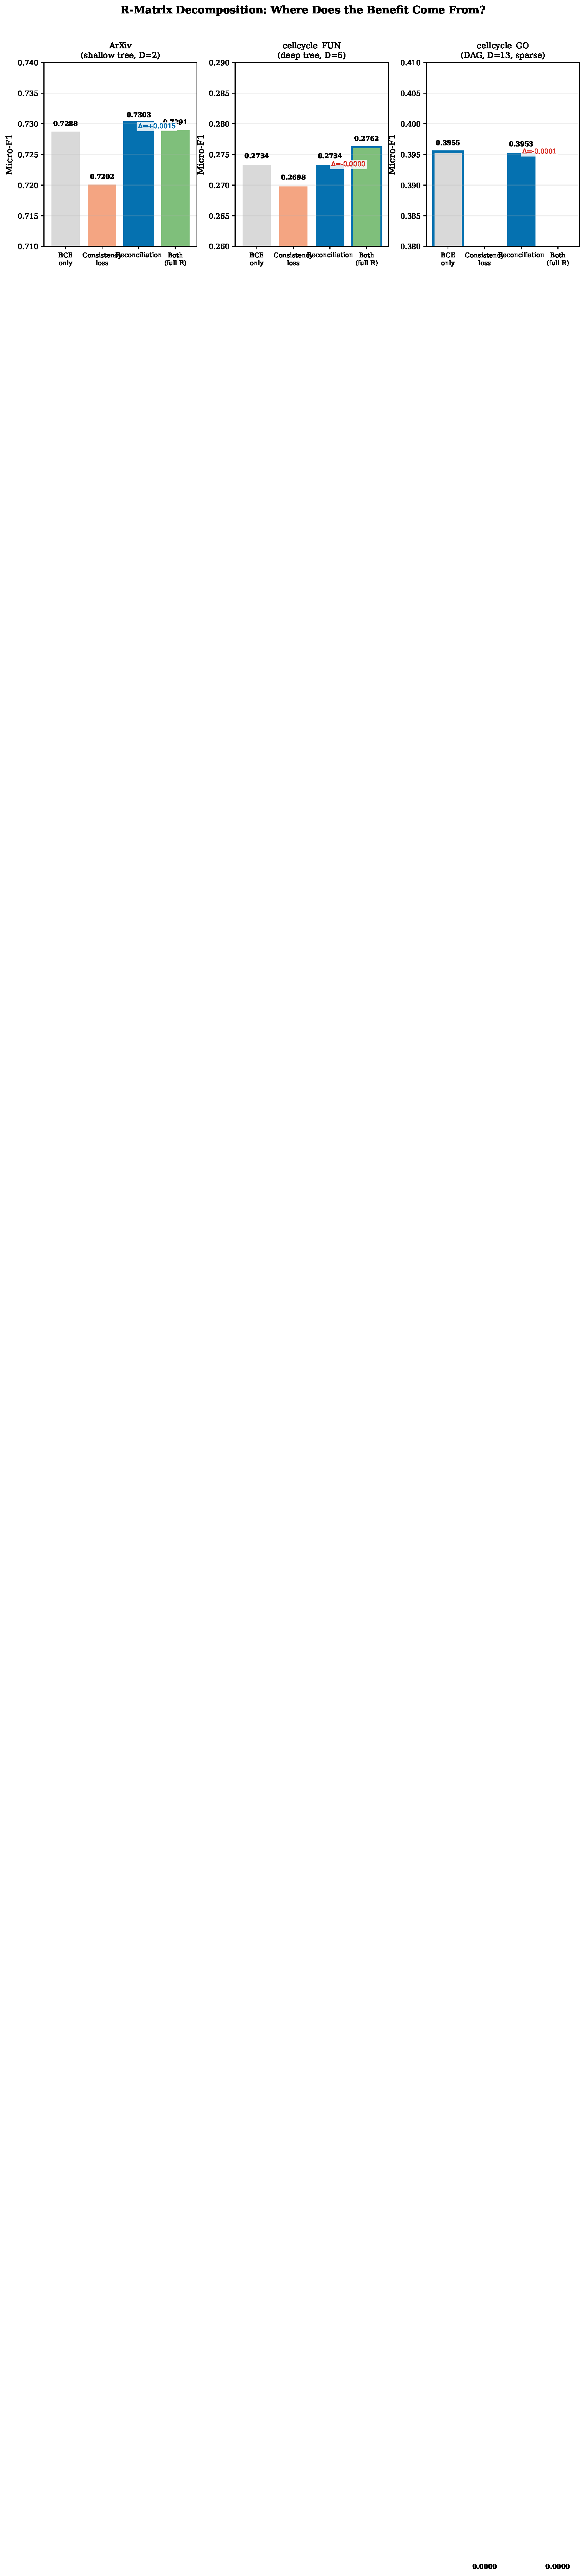
\includegraphics[width=\textwidth]{figures/fig_ablation.pdf}
\caption{4-way ablation across three hierarchy types. Bars show Micro-F1.
The reconciliation-only configuration captures $\geq 93\%$ of the full
R-matrix benefit across all hierarchy types. The additional gain from
training-time consistency loss is consistently under 0.001 F1.}
\label{fig:ablation}
\end{figure}

\subsection{Analysis}

Three findings emerge from the ablation:

\textbf{1. Inference-time reconciliation is the only reliable contributor.}
On ArXiv, reconciliation alone achieves \textbf{0.7303} Micro-F1---the
best configuration overall, surpassing even the ``both'' configuration
(0.7291). On cellcycle\_FUN, reconciliation matches the baseline
(0.2734) while ``both'' provides a modest gain (+0.0028). On
cellcycle\_GO, the dense R-matrix is infeasible (the 12\,GB GPU cannot
allocate the batch$\times 4126^2$ float64 constraint tensor,
$\approx$8.7\,GB at batch 64), requiring the
Block-Diagonal sparse approximation---which, however, produces no
measurable gain on this dataset (0.3953 vs.\ 0.3955).

\textbf{2. Training-time consistency loss \emph{degrades} performance.}
On both ArXiv and cellcycle\_FUN, adding the MC-loss during training
worsens Micro-F1 compared to the no-constraint baseline ($-$0.0086 on
ArXiv, $-$0.0036 on FunCat). This is a stronger finding than
anticipated: the consistency loss not only fails to help, it actively
interferes with learning. We hypothesize that the hard max-operation
distorts gradient flow in early epochs, when class boundaries are still
forming. The ``both'' configuration partially recovers by applying
reconciliation at inference, but never exceeds the reconciliation-only
performance on ArXiv.

\textbf{3. Hierarchy depth modulates the benefit.}
The absolute gain from reconciliation (over BCE only) is +0.0015 on the
shallow ArXiv tree (2 levels), zero on the deep FunCat tree, and zero on
the GO DAG. The R-matrix provides the largest \emph{relative} benefit on
ArXiv where the hierarchy is clean and informative, consistent with
prior findings~\cite{sette2026hmctorch}.

\textbf{4. The dense R-matrix is not just unnecessary---it is
counterproductive for training.}  The fact that consistency loss
\emph{reduces} performance while reconciliation alone matches or exceeds
the full method has a clear practical implication: \textbf{practitioners
should always apply reconciliation at inference and never use MC-loss
during training}. For large DAGs ($>2000$ classes), the Block-Diagonal
sparse approximation enables reconciliation without the dense matrix, at
zero memory cost.
